\documentclass[12pt, a4paper, openany]{book}
\usepackage{../generalStyle}
\usepackage{enumitem}

\graphicspath{ {./img/} }
\def\arraystretch{2} %define table vertical spacing
%\setlist{nolistsep,leftmargin=*} %remove list spacing
\newcolumntype{Y}{>{\centering\arraybackslash}X} %new tabularx centered X column  

\begin{document}
\title{CheatSheet di Analisi Matematica}

\author{
	Fabio Ferrario\\
	\small{\href{https://t.me/fefabo}{@fefabo}}
}
\date{2022/2023}

\maketitle

\tableofcontents

\section*{Insiemistica}

Dati un elemento $m$ e un insieme $A$:
\begin{itemize}
	\item \textbf{Massimo/Minimo}: $m$ si dice massimo/minimo di $A$ se esso \emph{Appartiene ad $A$} ed é il piú grande/piccolo elemento di $A$. 
	\item \textbf{Maggiorante/Minorante}: $m$ si dice maggiorante/minorante di $A$ se é \emph{Maggiore/Minore o uguale} di ogni elemento di $A$.
\end{itemize}

\chapter{Studio di Funzione}
Nello studio di funzione bisogna fare:
\begin{itemize}
	\item Definizione del Dominio
	\item Intersezione con gli Assi (Segno di $f(x)$)
	\item Limiti ai punti di frontiera e Asintoti
	\item Derivata, Monotonia e Estremanti
	\item Derivata Seconda, Concavià/Convessità
\end{itemize}
In particolare:

\section{Definizione del Dominio}
In una funzione il dominio ha i seguenti limiti:\\
\begin{tabular}{ l|l }
	Denominatore    & $\neq 0$                                 \\
	Logaritmo       & Argomento $>0$                           \\
	Radice$^n$      & Argomento $\geq 0$ (\emph{sse $n$ pari}) \\
	$[f(x)]^{g(x)}$ & $f(x)>0$
\end{tabular}

\section{Limiti ai punti di frontiera e Asintoti}
Trovato il dominio, bisogna trovare \emph{i limiti ai punti di frontiera},
quindi trovare i limiti in ogni punto in cui il dominio si interrompe (sia da destra che da sinistra) e eventualmente a $\pm \infty$.

\subsection{Asintoti}
Trovati tutti i limiti, se trovi:
\begin{itemize}
	\item $\limite{x}{\alpha^\pm} f(x) = \pm \infty \implies$ Asintoto \emph{Verticale}.
	\item $\limite{x}{\pm \infty} f(x) = l \implies$ Asintoto \emph{Orizzontale} (di equazione $y=l$)
\end{itemize}
Bisogna anche controllare la presenza di \textbf{Asintoti Obliqui}:
\begin{itemize}
	\item $m = \limite{x}{\pm \infty} \frac{f(x)}{x} \implies$ se $m$ \emph{esiste e non è nullo} trovo $q$:
	\item $q = \limite{x}{\pm \infty} [f(x) - mx]\implies$  se $q$ esiste allora $y=mx+q$ è \emph{asintoto obliquo}
\end{itemize}

\section{Derivata, Monotonia e Estremanti}
La monotonia di una funzione si calcola \emph{ponendo $f'(x)>0$.}
Nei punti in cui la derivata è positiva, la funzione è \textbf{Crescente}, nei punti in cui è negativa la funzione è \textbf{Decrescente}
\subsection{Punti di estremo} I punti in cui la derivata cambia direzione sono punti di estremo (max/min).
Se il punto di estremo è il più grande/piccolo di tutta la funzione, allora sono Assoluti.

\section{Derivata Seconda, Concavià/Convessità}
Derivando la derivata prima si trova la derivata seconda, il cui segno da informazioni sulla Concavià e Convessità della funzione.
\begin{itemize}
	\item $-$ conc$\mathcal{A}$va $\cap \implies f''(x)$ positiva
	\item $+$ con$\mathcal{V}$essa $\cup \implies f''(x)$ negativa
\end{itemize}

\section{Altri elmenti di studio di una funzione}
\subsection{Retta Tangente al grafico}
Se viene chiesta la retta tangente al grafico in $x_0$:\\
trova $y=mx + q$ ponendo:
\begin{itemize}
	\item $m=f'(x_0)$
	\item $q=f(x_0)-f'(x_0)\cdot x_0$
\end{itemize}

\subsection{Punti di Discontinuità}
I punti in cui una funzione non é continua si classificano nel seguente modo:
\begin{enumerate}
	\item Prima specie (Salto): i limiti dx e sx di $x_0$ esistono finiti ma sono diversi.
	\item Seconda spece (Essenziale): Almeno uno dei limiti è inifinito o non esiste.
	\item Terza Spece (Eliminabile): il limite di $x_0$ esiste finito ma è diverso da $f(x_0)$ o non esiste.
\end{enumerate}

\subsection{Funzioni Pari/Dispari}
\small{(serve solo per le crocette)}
\begin{itemize}
	\item $-$ Dispari $\implies f(-x)=-f(x)$
	\item $+$ Pari $\implies f(-x)=f(x)$
\end{itemize}
\paragraph*{Paritá e disparitá di funzioni note}

$\sin(x)$ è \emph{Pari}, \emph{Decrescente} in $[0,\pi]$ e \emph{Crescente} in $[\pi,2\pi]$.
\\$\cos(x)$ è \emph{Pari}, \emph{Crescente} in $[0,\pi]$ e \emph{Decrescente} in $[\pi,2\pi]$.


\chapter{Studio dei Limiti}

\section{Limiti Notevoli}
É importante ricordarsi questi limiti notevoli, visto che sono generalmente il modo piú rapido di risolvere i limiti

\begin{tabularx}{\textwidth}{ |X|X| }
	\hline
	Logaritmo naturale        & $\limite{x}{0} \frac{\ln(1+x)}{x} = 1 $                   \\
	\hline
	Logaritmo con base $a$    & $\limite{x}{0} \frac{\log_a(1+x)}{x} = \frac{1}{\ln(a)} $ \\
	\hline
	$f$ Esponenziale          & $\limite{x}{0} \frac{e^x-1}{x} = 1$                       \\
	\hline
	$f$ Esponenziale base $a$ & $\limite{x}{0} \frac{a^x-1}{x} = \ln(a)$                  \\
	\hline
	Costante e Frazione       & $\limite{x}{0}\frac{ax -1}{x} = \ln(a)$                   \\
	\hline
	Seno                      & $\limite{x}{0}\frac{\sin(x)}{x} = 1$                      \\
	\hline
	Coseno                    & $\limite{x}{0} \frac{1-\cos(x)}{x^2} = \frac{1}{2} $      \\
	\hline
	\hline
	$\ln(x)$                  & $\limite{x}{0} ln(x) = -\infty $                          \\ % 0 %perchè avevo messo 0? $\\
	\hline
\end{tabularx}

\pagebreak

\section{Equivalenze Asintotiche}
\definizione{
	\underline{\textbf{Equivalenza Asintotica} tra funzioni}: Se il limite del rapporto di $f(x)$ e $g(x)$ é uguale a 1 allora $f$ e $g$ sono asintoticamente equivalenti
	per $x\to x_0$.
	\[
		\lim_{x\to x_0} \frac{f(x)}{g(x)} = 1 \implies f(x) \sim g(x) \text{ per } x\to x_0 
	\]
	}
In particolare, alcune equivalenze note sono:
\\\begin{tabularx}{\textwidth}{|X|XYX|}
	\hline
	\multicolumn{4}{|c|}{\textbf{con \emph{x} $\to$ 0}} \\
	\hline
	\hline
	$\lim_{x\to 0}$ & $\sin x$           & $\sim$ & $x$                   \\
	\hline
	$\lim_{x\to 0}$ & $1-\cos x$         & $\sim$ & $\frac{1}{2}x^2$      \\
	\hline
	$\lim_{x\to 0}$ & $\tan x$           & $\sim$ & $x$                   \\
	\hline
	$\lim_{x\to 0}$ & $\ln(1+x)$         & $\sim$ & $x$                   \\
	\hline
	$\lim_{x\to 0}$ & $(1+x)^\alpha -1 $ & $\sim$ & $\alpha x$            \\
	\hline
\end{tabularx}

\paragraph{Osservazioni}
\begin{itemize}
	\item Le equivalenze asintotiche valcono anche per le Successioni
	\item Se (per esempio) $f(x) \to 0$, allora $sin(f(x)) \sim f(x)$, questo vale per tutte le equivalenze.
\end{itemize}

\subsection{O-Piccolo}
Una funzione puó essere un 'o-piccolo' di un'altra.
\definizione{
	\underline{\textbf{$o$-piccolo}}: 
	Se il limite del rapporto di $f(x)$ su $g(x)$ è uguale a $0$ allora $f(x)$ è $o$-piccolo di $g(x)$ per $x\to x_0$.
   $$lim_{x\to x_0} \frac{f(x)}{g(x)} = 0 \implies f(x) = o g(x)\text{ per } x\to x_0 $$
   \small{Questa proprietá NON é commutativa.}
}
Nota che per $x_0$ si intende un valore arbitrario che può essere anche 0 o $\pm \infty$.

\pagebreak

\section{Gerarchie di Infiniti}
In situazioni di indecisione del tipo $[\infty \pm \infty]$ 'vince' l'infinito piú forte.
\\In generale, la scala é la seguente:

\begin{center}
	\[ \log_ax\ll x^b\ll c^x\ll x! \ll x^x \]
\end{center}
\nb{
	\begin{itemize}
		\item 	$\sqrt{x} \gg \ln(x) $
		\item $x \ln (x) \gg \sqrt{x}$
	\end{itemize}
}

\section{Forme di indecisione}
In alcuni casi ci potremmo trovare delle Forme di indecisione che ci obbligano a usare altri metodi per risolvere i limiti.\\
\begin{tabularx}{\textwidth}{|l|X|}
	\hline
	\multicolumn{2}{|c|}{
		$[\frac{0}{0}]$ $[\frac{\infty}{\infty}]$ $[1^\infty]$ $[\infty - \infty]$ $[\infty \cdot 0]$ $[0^0]$ $[\infty^0]$
	}                                                                                       \\
	\hline
	\multicolumn{2}{|X|}{
		\small{Tutte le forme possono essere risolte usando \textbf{Limiti Notevoli} e \textbf{Trucchi algebrici} per ricondursi ad essi.
			In particolare però, questi si risolvono usando anche:}
	}                                                                                       \\
	\hline
	$[\frac{0}{0}]$           & Conf. infinitesmi | Scomp/Racc/Semp | De l'Hopital          \\
	\hline
	$[\frac{\infty}{\infty}]$ & Conf. infinti | Scomp/Racc/Semp | De l'Hopital              \\
	\hline
	$[1^\infty]$              & Identità Logaritmo-Esponenziale                             \\
	\hline
	$[\infty - \infty]$       & Riconduzione a $\frac{0}{0}$ o $\frac{\infty}{\infty}$      \\
	\hline
	$[\infty \cdot 0]$        & Razionalizzazione inversa | Prodotti notevoli al contrario  \\
	\hline
	$[0^0]$ / $[\infty^0]$    & Conf. infiniti/infinitesimi|Identità Logaritmo-Esponenziale \\
	\hline
\end{tabularx}

\section{Teoremi per i Limiti}
\subsection{Teorema di de l'Hopital}
Il teorema di de l'Hopital è utile per risolvere le forme di indecisione del tipo $[\frac{0}{0}]$ e $[\frac{\infty}{\infty}]$:

\definizione{
	Siano $f(x)$ e $g(x)$ due funzioni definite in un intorno di $x_0$.
	\\Siano anche derivabili in un intorno di $x_0$ (privato eventualmente di ${x_0}$),
	con $g'(x)\neq 0$, e sia $lim_{x\to x_0} f(x) = lim_{x\to x_0} g(x) = 0$ (o $\pm \infty$).
	\[
	\text{Se } lim_{x\to x_0} \frac{f'(x)}{g'(x)} = l \implies lim_{x\to x_0} \frac{f(x)}{g(x)} = l
	\]
}

\subsection{Teorema del Confronto} Se ho $x \rightarrow +\infty$ e ho $\sin$ o  $\cos$ potrei dover usare
il teorema del confronto dato che $\sin$ e $\cos$ (NB solo per $x \rightarrow +\infty$)
sono delle costanti che oscillano tra $-1$ e $1$.

\chapter{Successioni}

\section{Limiti di Successioni}

\subsection{Criterio del Rapporto per i Limiti di successioni}
Se dobbiamo trovare il limite di una successione in cui sono presenti $n!$ o $n^n$
potrebbe essere utile usare il criterio del rapporto, che ci permette di sapere se la successione
\emph{Converge a Zero o Diverge a $+\infty$}

\paragraph*{Semplificare $(n+1)$}
Quando usiamo il criterio del rapporto ci capita spesso di incontrare alcune forme con $n+1$ che non sono immediate da semplificare:
\begin{itemize}
	\item $(n+1)! = (n+1) \cdot n!$
	\item $(n+1)^n = (n+1)^n \cdot (n+1)$
	\item $(n+1)^{\alpha} = n^{\alpha} \cdot (1+\frac{1}{n})^\alpha$ 
\end{itemize}
Una piccola \textbf{osservazione}:
\\Se troviamo $(n+1)^n = (n+1)^n \cdot (n+1)$, allora abbiamo anche $(n+1)^{n} = n^{n} \cdot (1+\frac{1}{n})^ n$.
Sappiamo inoltre che $\lim_{n\to +\infty}(1+\frac{1}{n})^n = e$.
\\Quindi $\lim_{n\to +\infty}(n+1)^n = ... = n^n \cdot e \cdot (n+1)$

\subsection{Teorema di Permanenza del Segno}
Il Teorema di Permanenza del Segno per il limite di una successione enuncia qunato segue:
\definizione{
	Sia $a_n \to l$. allora:
	\begin{itemize}
		\item Se $l>0$ o $l=+\infty$, allora $a_n>0$ definitivamente.
		\item Se $a_n>0$, allora $l\geq 0$.
	\end{itemize}
}


\chapter{Serie}
\section{Serie Note}

\paragraph*{Serie Telescopica}
\begin{equation*}
	\serie{1}{+\infty} (a_n - a_{n+k})
	\text{ Oppure: }
	\serie{1}{+\infty} (a_{n+k} - a_n)
\end{equation*}

\subparagraph{Come si risolve una serie telescopica}
É necessario applicare la definzione di serie, cioè la successione delle somme
parziali. Devo quindi manualmente sostituire n=1, n=2, n=3, ...
fino a quando non riconosco il pattern della serie.
\\ \emph{Ricordati di non semplificare Numeratore e Denominatore!},
mantenendo i numeri sostituiti sarà più facile scrivere il carattere della serie.


\paragraph*{Serie Geometrica}
\begin{equation*}
	\serie{0}{+\infty} q^n \begin{cases}
		\text{Diverge}    & q\geq 1  \\
		\text{Converge}   & -1<q<1   \\
		\text{Irregolare} & q\leq -1
	\end{cases}
\end{equation*}
\subparagraphmark{Somma di una Serie Geometrica Convergente} Se una serie geometrica converge ($-1<q<1$),
la somma si calcola:
\[
	\serie{0}{+\infty} q^n = \frac{1}{1-q}
\]

\paragraph*{Serie Armonica Generalizzata}
\begin{equation*}
	\sum \frac{1}{n^\alpha} \begin{cases}
		\text{Diverge}  & \alpha\leq 1 \\
		\text{Converge} & \alpha> 1
	\end{cases}
\end{equation*}

\paragraph*{Serie Armonica Logaritmica}
\begin{equation*}
	\sum \frac{1}{n^\alpha \log^\beta(n)}
	\begin{cases}
		\text{Converge} & \alpha > 1 \wedge \forall \beta \\
		\text{Converge} & \alpha = 1 \wedge \beta > 1     \\
		\text{Diverge}  & \alpha = 1 \wedge \beta \leq 1  \\
		\text{Diverge}  & \alpha < 1 \wedge \forall \beta
	\end{cases}
\end{equation*}


\section{Criteri di Convergenza}

\definizione{
	Condizione \textbf{Necessaria non Sufficiente} per la convergenza:\\
	Il Limite della successione del termine generale $a_n$ deve essere \emph{Inifinitesimo}.
	\[
		\sum_{n=1}^{+\infty} a_n \text{ converge} \implies \lim_{n\to +\infty} a_n = 0
	\]
}

\subsection*{Serie Positive def$^{\text{ \underline{nte}}}$}
Se $a_n$ è def$^{\text{ \underline{nte}}} \geq 0$ uso:
\paragraph*{Criterio del Rapporto} 
\[
	\limite{n}{+\infty} \frac{a_{n+1}}{a_n} = l
	\begin{cases}
		\text{Converge} &  l<1\\
		\text{Diverge} & l>1\\
		\text{Criterio inconclusivo} & l=1
	\end{cases}
\]

\paragraph*{Criterio della Radice} 
\[
	\limite{n}{+\infty} \sqrt[n]{a_n} = l
	\begin{cases}
		\text{Converge} &  l<1\\
		\text{Diverge} & l>1\\
		\text{Criterio inconclusivo} & l=1
	\end{cases}
\]

\paragraph*{Criterio del Confronto}
$a_n\leq b_n$ definitivamente $\implies$
\begin{itemize}
	\item se $b_n$ Converge $\implies$  $a_n$ Converge
	\item se $a_n$ Diverge $+\infty$ $\implies$ $b_n$ Diverge $+\infty$
\end{itemize}

\subsection*{Serie con Segno Alterno}
Se $a_n$ è a segno \textbf{Alterno}: 

\paragraph{Criterio della Assoluta Convergenza}.\\
$\sum a_n$ \textbf{converge assolutamente} se converge $\sum |a_n|$.\\
Se una serie converge assolutamente, allora converge.

\paragraph{Criterio di Leibniz}
DA SCRIVERE

\chapter{Calcolo Differenziale}



\section{Definizione di derivata e il Rapporto Incrementale}
\paragraph*{il Rapporto incrementale} Di una funzione è alla base della definizone di derivata, ed è così definito:

\[ 
	\frac{\Delta y}{ \Delta x}\frac{f(x_0+h)-f(x_0)}{h} 
\]
\definizione{
	La \textbf{derivata di una funzione} in un punto è il limite del rapporto incrementale della
	funzione nel punto al tendere dell'incremento a zero.
	
	\[ 
		f'(x_0) = \lim_{h\to 0} \frac{\Delta y}{ \Delta x}\frac{f(x_0+h)-f(x_0)}{h} 
	\]
}




\section{Tecniche e Metodi di derivazione}
Alcune funzioni sono facilmente derivabili:\\
\begin{tabularx}{\textwidth}{|Y|c|c|}
	\hline
	\textbf{Nome}           & \textbf{Funzione} & \textbf{Derivata}     \\
	\hline
	\hline
	Seno                    & $\sin x$          & $\cos x$              \\
	\hline
	Coseno                  & $\cos x$          & $-\sin x$             \\
	\hline
	Arcotangente            & $\arctan$         & $\frac{1}{1+x^2}$     \\
	\hline
	Logaritmo               & $\ln(x) $         & $\frac{1}{x}$         \\
	\hline
	Esponenziale            & $e^x$             & $e^x$                 \\
	\hline
	Esponenziale (negativo) & $e^{-x}$          & $ -e^{-x}$            \\
	\hline
	1 su $x^2$              & $\frac{1}{x^2}$   & $-\frac{2}{x^3}$      \\
	\hline
	$x$ alla $\alpha$       & $x^\alpha$        & $\alpha x^{\alpha-1}$ \\
	\hline
\end{tabularx}

\subsection{Derivate Composte}

\begin{tabularx}{\textwidth}{|l|Y|Y|}
	\hline
	Funzione composta & $f(g(x))$           & $ f'(g(x))\cdot g'(x)$                                \\
	\hline
	Prodotto     & $f(x)\cdot g(x)$    & $f'(x)\cdot g(x) + g'(x)\cdot f(x)$                   \\
	\hline
	Divisione    & $\frac{f(x)}{g(x)}$ & $\frac{f'(x)\cdot g(x) - g'(x) \cdot f(x)}{[g(x)]^2}$ \\
	\hline
\end{tabularx}

\subsection{Derivata dell'inversa di una funzione}
Dati:\\
$y_o$ e $f(x)$, avendo $g(x) = f^{-1}(x)$ allora:
Per calcolare $g'(y_0)$
\begin{enumerate}
	\item trovo $x_0$ ponendo $y_0=f(x)$
	\item trovo $g'(y_0)=\frac{1}{f'(x_0)}$
\end{enumerate}

\section{Sviluppi di Taylor e McLaurin}

\subsection{Tayolr}
Lo sviluppo di taylor di una funzione in un punto, se esiste permette di approssimare la funzione in un polinomio.
Essendo un'approssimazione, può anche essere usato per lo studio dei limiti.


\paragraph{Polinomio di Taylor} Il polinomio di Taylor di una funzione di grado $k$ e centrato in $x_0$ è così definito:
$$P_k(x)=f(x_0)+f'(x_0)(x-x_0) + \frac{1}{2}f''(x_0)(x-x_0)^2 +... + \frac{1}{k!}f^{(k)}(x_0)(x-x_0)^k$$

\paragraph*{Lo sviluppo} Se viene richiesto lo Sviluppo di Taylor di f(x), avendo $P(x)$ come Polinomio di Taylor di $f(x)$ allora:
\\Sviluppo di taylor di grado $k$: $f(x) \simeq P(x) + o(x^k)$.

\subsection{McLaurin}
Se uno sviluppo di Taylor è centrato in $x_0=x$, allora può essere semplificato con il polinomio di Mclaurin.
\paragraph*{Polinomio di Mclaurin} di grado $k$:
$$P_k(x)=f(0)+f'(0)x+\frac{1}{2}f''(0)x^2+...+\frac{1}{k!}f^{(k)}(0)x^k$$




\chapter{Calcolo Integrale}
\paragraph*{Condizione di integrabilità} Per l'integrabilità di una funzione su un intervallo la condizione
che essa sia \emph{continua è sufficiente ma non necessaria}
\begin{multicols}{3}
	\paragraph*{\underline{Primitive elementari}}
	Funzioni il cui integrale è immediatamente calcolabile.
	\columnbreak
	\begin{tabularx}{0.7\textwidth}{ |Y|Y| }
		\hline
		\textbf{Funzione} & \textbf{Primitiva}    \\
		\hline
		$k$               & $kx$                  \\
		$x^a$,$a\neq-1$   & $\frac{x^{a+1}}{a+1}$ \\
		$\frac{1}{x}$     & $\log|x|$             \\
		$\sin x$          & $-\cos x$             \\
		$\cos x $         & $\sin x$              \\
		$a^x$             & $\frac{a^x}{\log a}$  \\
		\hline
		$e^{-x}$          & $-e^{-x}$             \\
		$\frac{1}{x^2+1}$ & $\arctan (c)$         \\
		\hline
	\end{tabularx}
\end{multicols}

\paragraph*{Proprietà degli integrali}
\begin{itemize}
	\item Somma di integrali: $\int f(x)+g(x) dx = \int f(x) dx + \int g(x) dx$
	\item Costante moltiplicativa $\int k \cdot f(x) = k \int f(x)$
\end{itemize}
\subsection*{I metodi di risoluzione}
\paragraph*{Integrazione per Parti}
$$\int f(x)g'(x)dx = f(x)g(x)-\int f'(x)g(x)dx$$
\begin{center}
	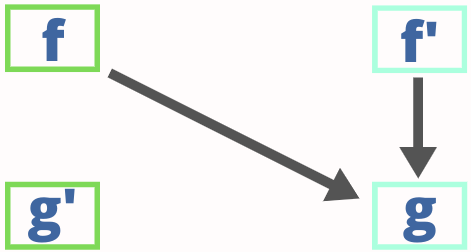
\includegraphics[width=0.4\textwidth]{integrazione-per-parti.png}
\end{center}

\paragraph*{\underline{Integrazione per Sostituzione}}
\subparagraph*{\emph{Metodo Generale e Semplificato}} per itnegrali generali $f(x)$:
\\Trovo una funzione $g(x)$ \emph{Derivabile e Invertibile} da sostituire ad $x$.
\begin{enumerate}
	\item decido che $y=g(x)$
	\item Inverto $g(x)$ per isolare la x, ottenendo $x=g^{-1}(y)$
	\item Derivo entrambi i membri e aggiungo $dx$ e $dy$: $\to dx=(g^{-1})'(y)dy$
	\item all'interno di $f(x)$ sosdtituisco $g(x) \to y$ e $dx \to (g^{-1})'(y)dy$
	\item Risolvo l'integrale
	\item Sostiuisco $y \to g(x)$
\end{enumerate}
\subparagraph*{Metodo dalla definizione}: Abbiamo un integrale nella forma
$$\int f(g(x))g'(x) dx$$
\begin{enumerate}
	\item $y=g(x)\to dy=g'(y)dx$
	\item Sostituiamo per ottenere $\int f(y)dy$
	\item Calcolo l'integrale nella nuova variabile
	\item Sostituisco $y\to g(x)$
\end{enumerate}

\paragraph*{Formula Media Integrale}
Considerata f limitata e integrabile su un intervallo $[a,b]$
\begin{equation*}
	M(f,[a,b])=\frac{1}{b-a}\int_a^b f(x)dx
\end{equation*}

\section{Dimostrazioni per induzione}
Le due casistiche principali sono:
\begin{itemize}
	\item Dimostrazioni con la sommatoria $\sum$
	\item Dimostrazioni con disequazioni
\end{itemize}
\paragraph*{Ricorda} Devi sempre dimostrare che la formula è vera per $n+1$, quindi devi ricondurti a
ciò che hai a destra dell'equazione.

\subsection*{Dimostrazioni con la sommatoria}
In questo caso devo ricordarmi di ricondurmi al caso base estrando dalla sommatoria (n+1)
per ricondurmi alla sommatoria $\sum^n$ e poi sostituendo l'ipotesi induttiva
(la sommatoria che supponiamo vera). Così facendo posso ottenere ciò che ho a sinistra della
formula $\sum^{n+1}$.
\subsection*{Dimostrazioni con le disequazioni}
In questo caso devo ricordarmi che oltre a dover sostituire l'ipotesi induttiva nella disequazione
possono aggiungere numeri che mi possono servire a patto che abbia la certezza che questi numeri non
vadano in contraddizione con il segno della disequazione, quindi se ho $a>b$, aggiungendo numeri non deve succedere
che b diventi maggiore di a.
\paragraph*{Ricorda} Nell'ipotesi avrai una condizione (per esempio per $n>1$), ricordati che puoi e spesso
devi usarla per poter aggiungere numeri utili alla dimostrazione.


\end{document}